21. \begin{figure}[ht!]
\center{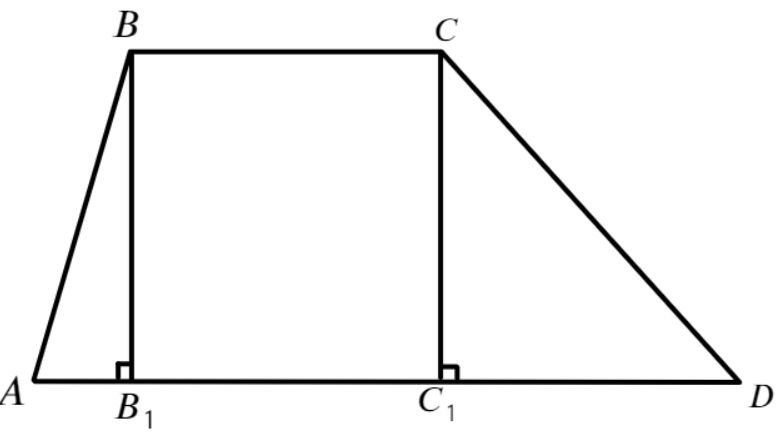
\includegraphics[scale=0.35]{g9-21.png}}
\end{figure}\\
Опустим высоты $BB_1$ и $CC_1.$ Пусть $AB=17$см, $BC=16$см, $CD=25$см, $AD=44$см, $AB_1=x.$ Тогда $C_1D=44-16-x=28-x$ и по теореме Пифагора имеем равенства
$17^2-x^2=BB_1^2=CC_1^2=25^2-(28-x)^2,\ 289-x^2=625-784+56x-x^2,\ 56x=448,\ x=8$см. Таким образом, $BB_1=\sqrt{289-64}=15$см и $S_{ABCD}=15\cdot\cfrac{16+44}{2}=450\text{ см}^2.$\\
